\documentclass[titlepage]{article}

\usepackage[english]{babel}
\usepackage{pdfpages} 
\usepackage{sidecap}
\usepackage{wrapfig}


%
\usepackage[top=1.5in, bottom=1.5in, left=2in, right=2in]{geometry}

\newcommand{\myparagraph}[1]{\paragraph{#1}\mbox{}\\}

\addtolength{\oddsidemargin}{-.875in}
\addtolength{\evensidemargin}{-.875in}
\addtolength{\textwidth}{1.75in}

\def \RoCM {Rotation Curve Modeler}

\begin{document}

\title{
\textbf{
Object Design Document}
\protect\\
for the
\protect\\
\textbf{
\RoCM\ (RoCM)}
\protect\\
{\small Version 2.0}}

\author{Robert Moss, Alex Clement}
\maketitle

\newpage
\tableofcontents{} 
\newpage

\section{Introduction}

\subsection{Object Design Trade-offs}

\subsubsection{Buy vs. Build}
There is no product in circulation that allows a user to plot all the existing theories that solve the rotation curve of galaxies. For this reason, we will have to build such a system, because buying it is not an option. In order to expedite the process of solving the rotation curve problem, a piece of software like RoCM will have to be created.
	

\subsubsection{Space vs. Speed}
Speed is a major priority for RoCM. The latency in updating each model will hinder the functionality of the application. RoCM 1.0 benchmarks extremely well with heavy computations. This gives light to RoCM 2.0 to continue to use JavaScript for the galactic models because the speed has not presented itself as an issue. The amount of space needed to hold the entire program will be negligible, because it will be held on an external server.

\subsubsection{Delivery Time vs. Functionality}
If the development of RoCM is behind schedule, certain features and models can be put on hold. The modularity of the design allows for this. Although, to get the full functionality of the tool, all the models will need to be implemented before it's release.

\subsubsection{Delivery Time vs. Quality}
If testing runs behind schedule, the software can still be released and updates can be released to fix bugs at a later date. As long as the core functionality of the rotation curve plotter and several models are provided, the product can be delivered.

\subsubsection{Files vs. Databases}
Files would not be as beneficial as a database because the data for RoCM is kept external from the user. A database would provide a sufficient structure to organize the galactic data and parameters. In using a file, users can theoretically edit and thus corrupt the file and the data inside. An "off site" database would be more secure and less likely to be modified.

\subsection{Interface Documentation Guidelines}
\textbf{\textit{Classes}, \textit{Interfaces} \& \textit{Packages}}: These names should be in \textit{Pascal Case}.
\begin{itemize}
	\item i.e.: CurvePlot, GalacticModel, ParamSlider
\end{itemize}
\textbf{\textit{Constants}}: All constants should be entirely in \textit{Upper Case}.
\begin{itemize}
	\item i.e.: MODEL, PARAMS 
\end{itemize}
\textbf{\textit{Functions}}: Identifier and Method names should be \textit{lowercase} and separated by an \textit{underscore}.
\begin{itemize}
	\item i.e.: get\_range(), update\_line()
\end{itemize}
\textbf{\textit{Local Variables}}: Variables should be in \textit{Camel Case}.
\begin{itemize}
	\item i.e.: data, errorBar, fileName
\end{itemize}

\subsection{Definitions, Acronyms, and Abbreviations}
\begin{itemize}
	\item Application Specific Definitions
	\begin{itemize}
		\item RoCM - Rotation Curve Modeler
		\item SOCM - Scholarly Observed Celestial Measurements
		\item RoCS - Rotation Curve Simulator
	\end{itemize}
	\item Industry Definitions
	\begin{itemize}
		\item WIT - Wentworth Institute of Technology
		\item ODD - Object Design Document
		\item JavaScript - A web based programming language.
		\item D3 - Data Driven Documents: A JavaScript library for data visualization.
		\item Ruby on Rails - A web development framework written in the Ruby programming language.
		\item JQuery - A JavaScript library for easy UI development.
		\item LaTeX - A document preparation system used widely throughout science and mathematics.
		\item SVG - Scalable Vector Graphics: A loss-less graphics format.
	\end{itemize}
	\item Technical Definitions
	\begin{itemize}
        \item MoND - Modification of Newtonian Dynamics
		\item TeVeS - Tensor-vector-scalar gravity
		\item MATLAB - A mathematical programming language (MATrix LABoratory).
		\item Mathematica - A mathematical programming language.
		\item DB - Database
        \item UI - User Interface
		\item GUI - Graphical User Interface
		\item HTML - HyperText Markup Language
		\item div - HTML tag to define a division in a document
        \item DOM - Document Object Model. A convention for representing and interacting with objects in HTML.
        \item API - Application Programming Interface
        \item km/s - Kilometers Per Second
        \item kpc - Kiloparsecs
	\end{itemize}
\end{itemize}

\section{Packages}
\subsection{Package Diagram}
\begin{center}
	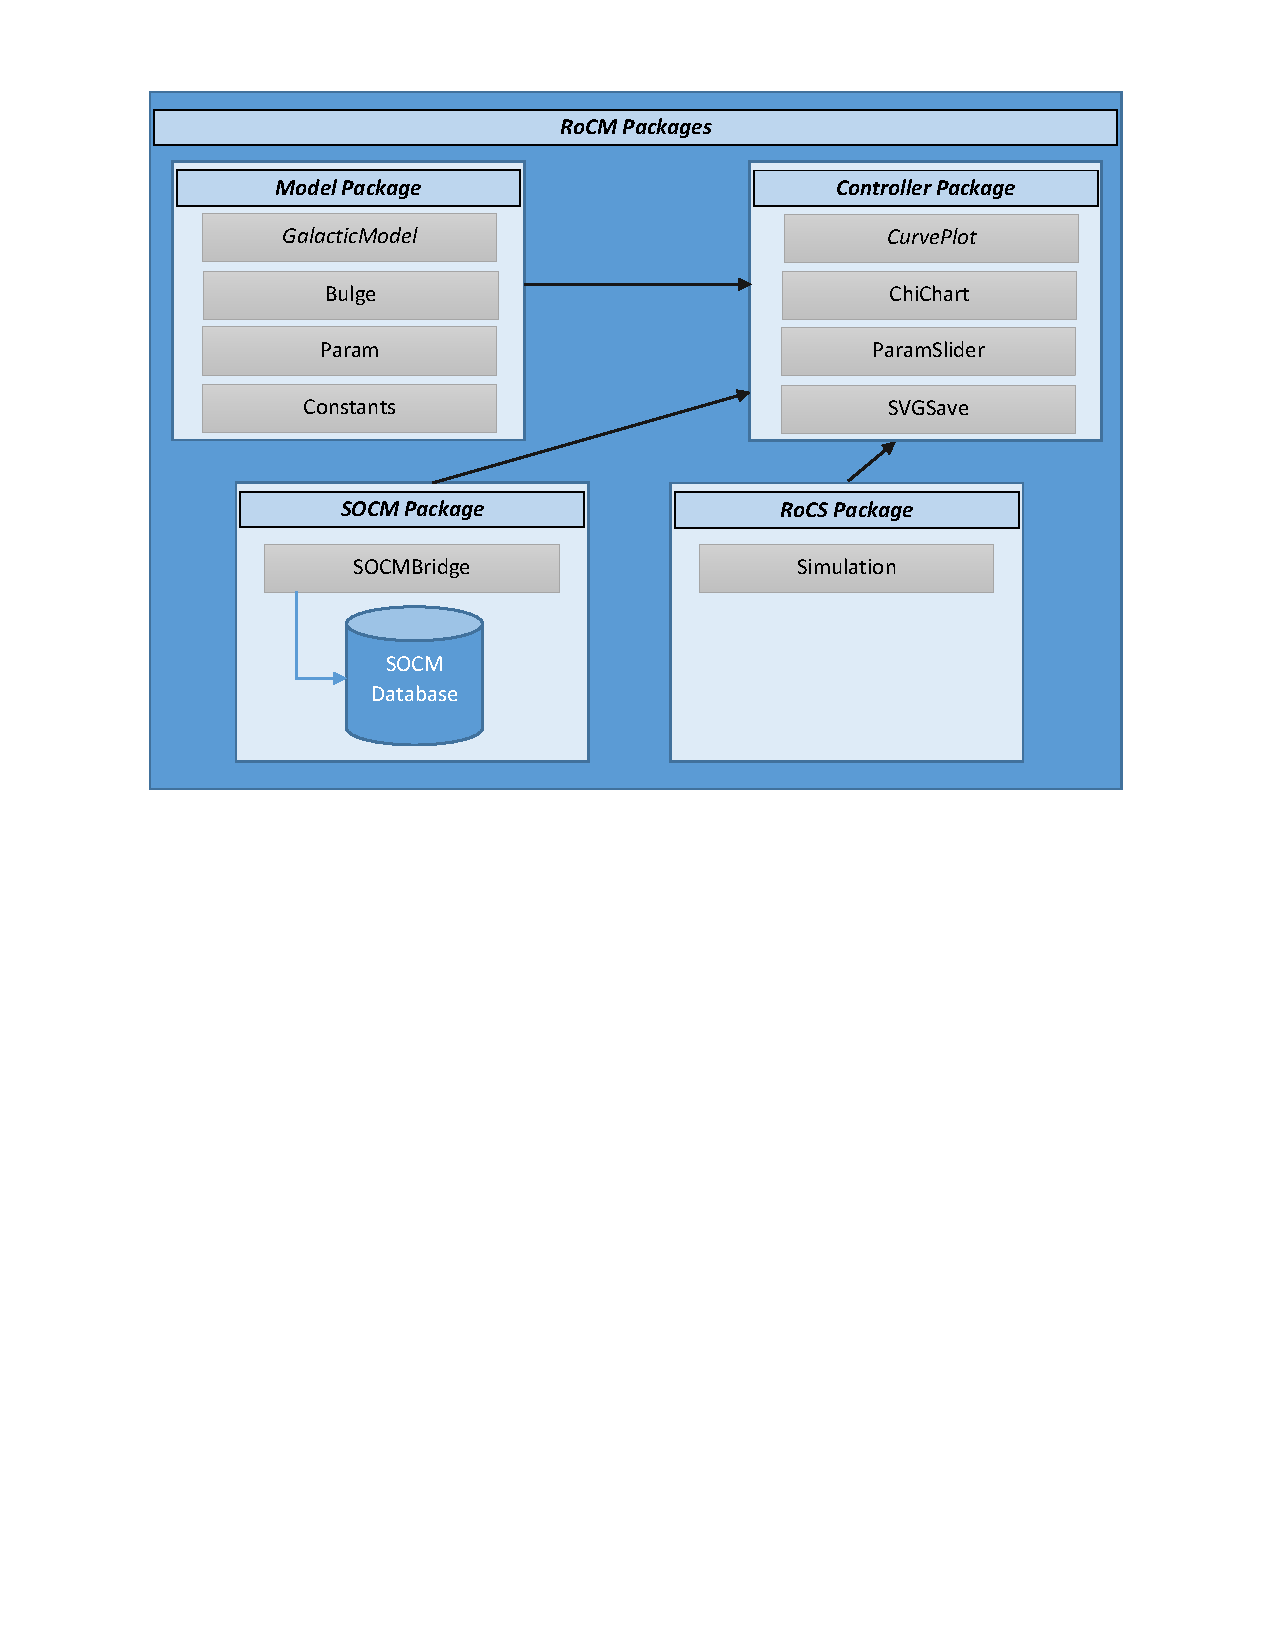
\includegraphics[trim={2cm 14cm 1cm 1cm},clip,scale=1]{package_diagram.pdf}
\end{center}

\newpage

\subsection{Package Definition}
\subsubsection{Model Package}
\begin{minipage}{\textwidth}
\begin{wrapfigure}{l}{0.45\textwidth}
  \vspace{-20pt}
  \begin{center}
	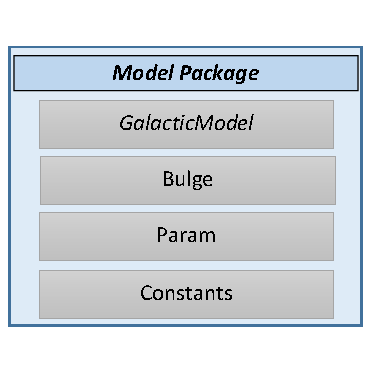
\includegraphics{model_package.pdf}
  \end{center}
\end{wrapfigure}
The model package will consist of the GalacticModel function set. It will include the Bulge contribution as a separate object. The Constants object will be initialized within this package because the GalacticModels are the only set of functions that use the Constants. The Param variable type will also be under this package. 
\end{minipage}

\vspace{+100pt}

\subsubsection{Controller Package}
\begin{minipage}{\textwidth}
\begin{wrapfigure}{l}{0.45\textwidth}
  \vspace{-20pt}
  \begin{center}
	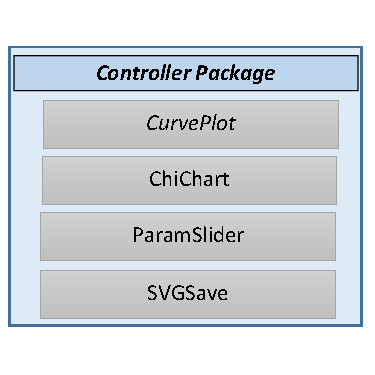
\includegraphics{controller_package.pdf}
  \end{center}
\end{wrapfigure}
The controller package will handle all of the graphing and curve plotting for RoCM. The CurvePlot object will deal solely with the data plotting and curve plotting functionality. The ChiChart histogram will generate it's own graph within this package. The ParamSlider object, which updates the CurvePlot and ChiChart, will be included in the controller package. Lastly, the SVGSave object which handles the conversion of the computed SVG elements into a static, savable, SVG file.
\end{minipage}

\vspace{+100pt}

\subsubsection{RoCS Package}
\begin{minipage}{\textwidth}
\begin{wrapfigure}{l}{0.45\textwidth}
  \vspace{-20pt}
  \begin{center}
	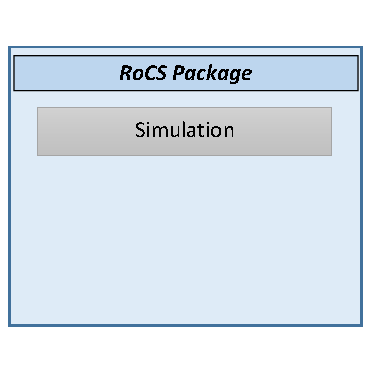
\includegraphics{rocs_package.pdf}
  \end{center}
\end{wrapfigure}
The RoCS package will handle all of the rotation curve simulation done in D3. The simulation function is the key component to this package. 
\end{minipage}

\vspace{+100pt}

\subsubsection{SOCM Package}
\begin{minipage}{\textwidth}
\begin{wrapfigure}{l}{0.45\textwidth}
  \vspace{-20pt}
  \begin{center}
	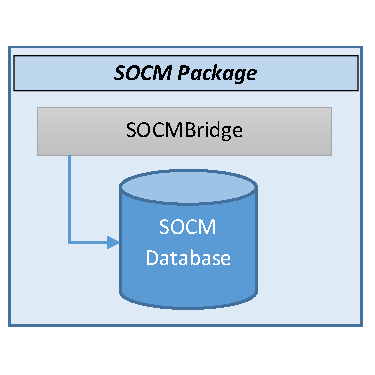
\includegraphics{socm_package.pdf}
  \end{center}
\end{wrapfigure}
The SOCM package is an entry point into the application. The SOCMBridge will query galactic data from the SOCM Database. All data retrieval will be handled within this package.
\end{minipage}

\vspace*{+100pt}

\section{Class Interface}
\subsection{Class Diagram}
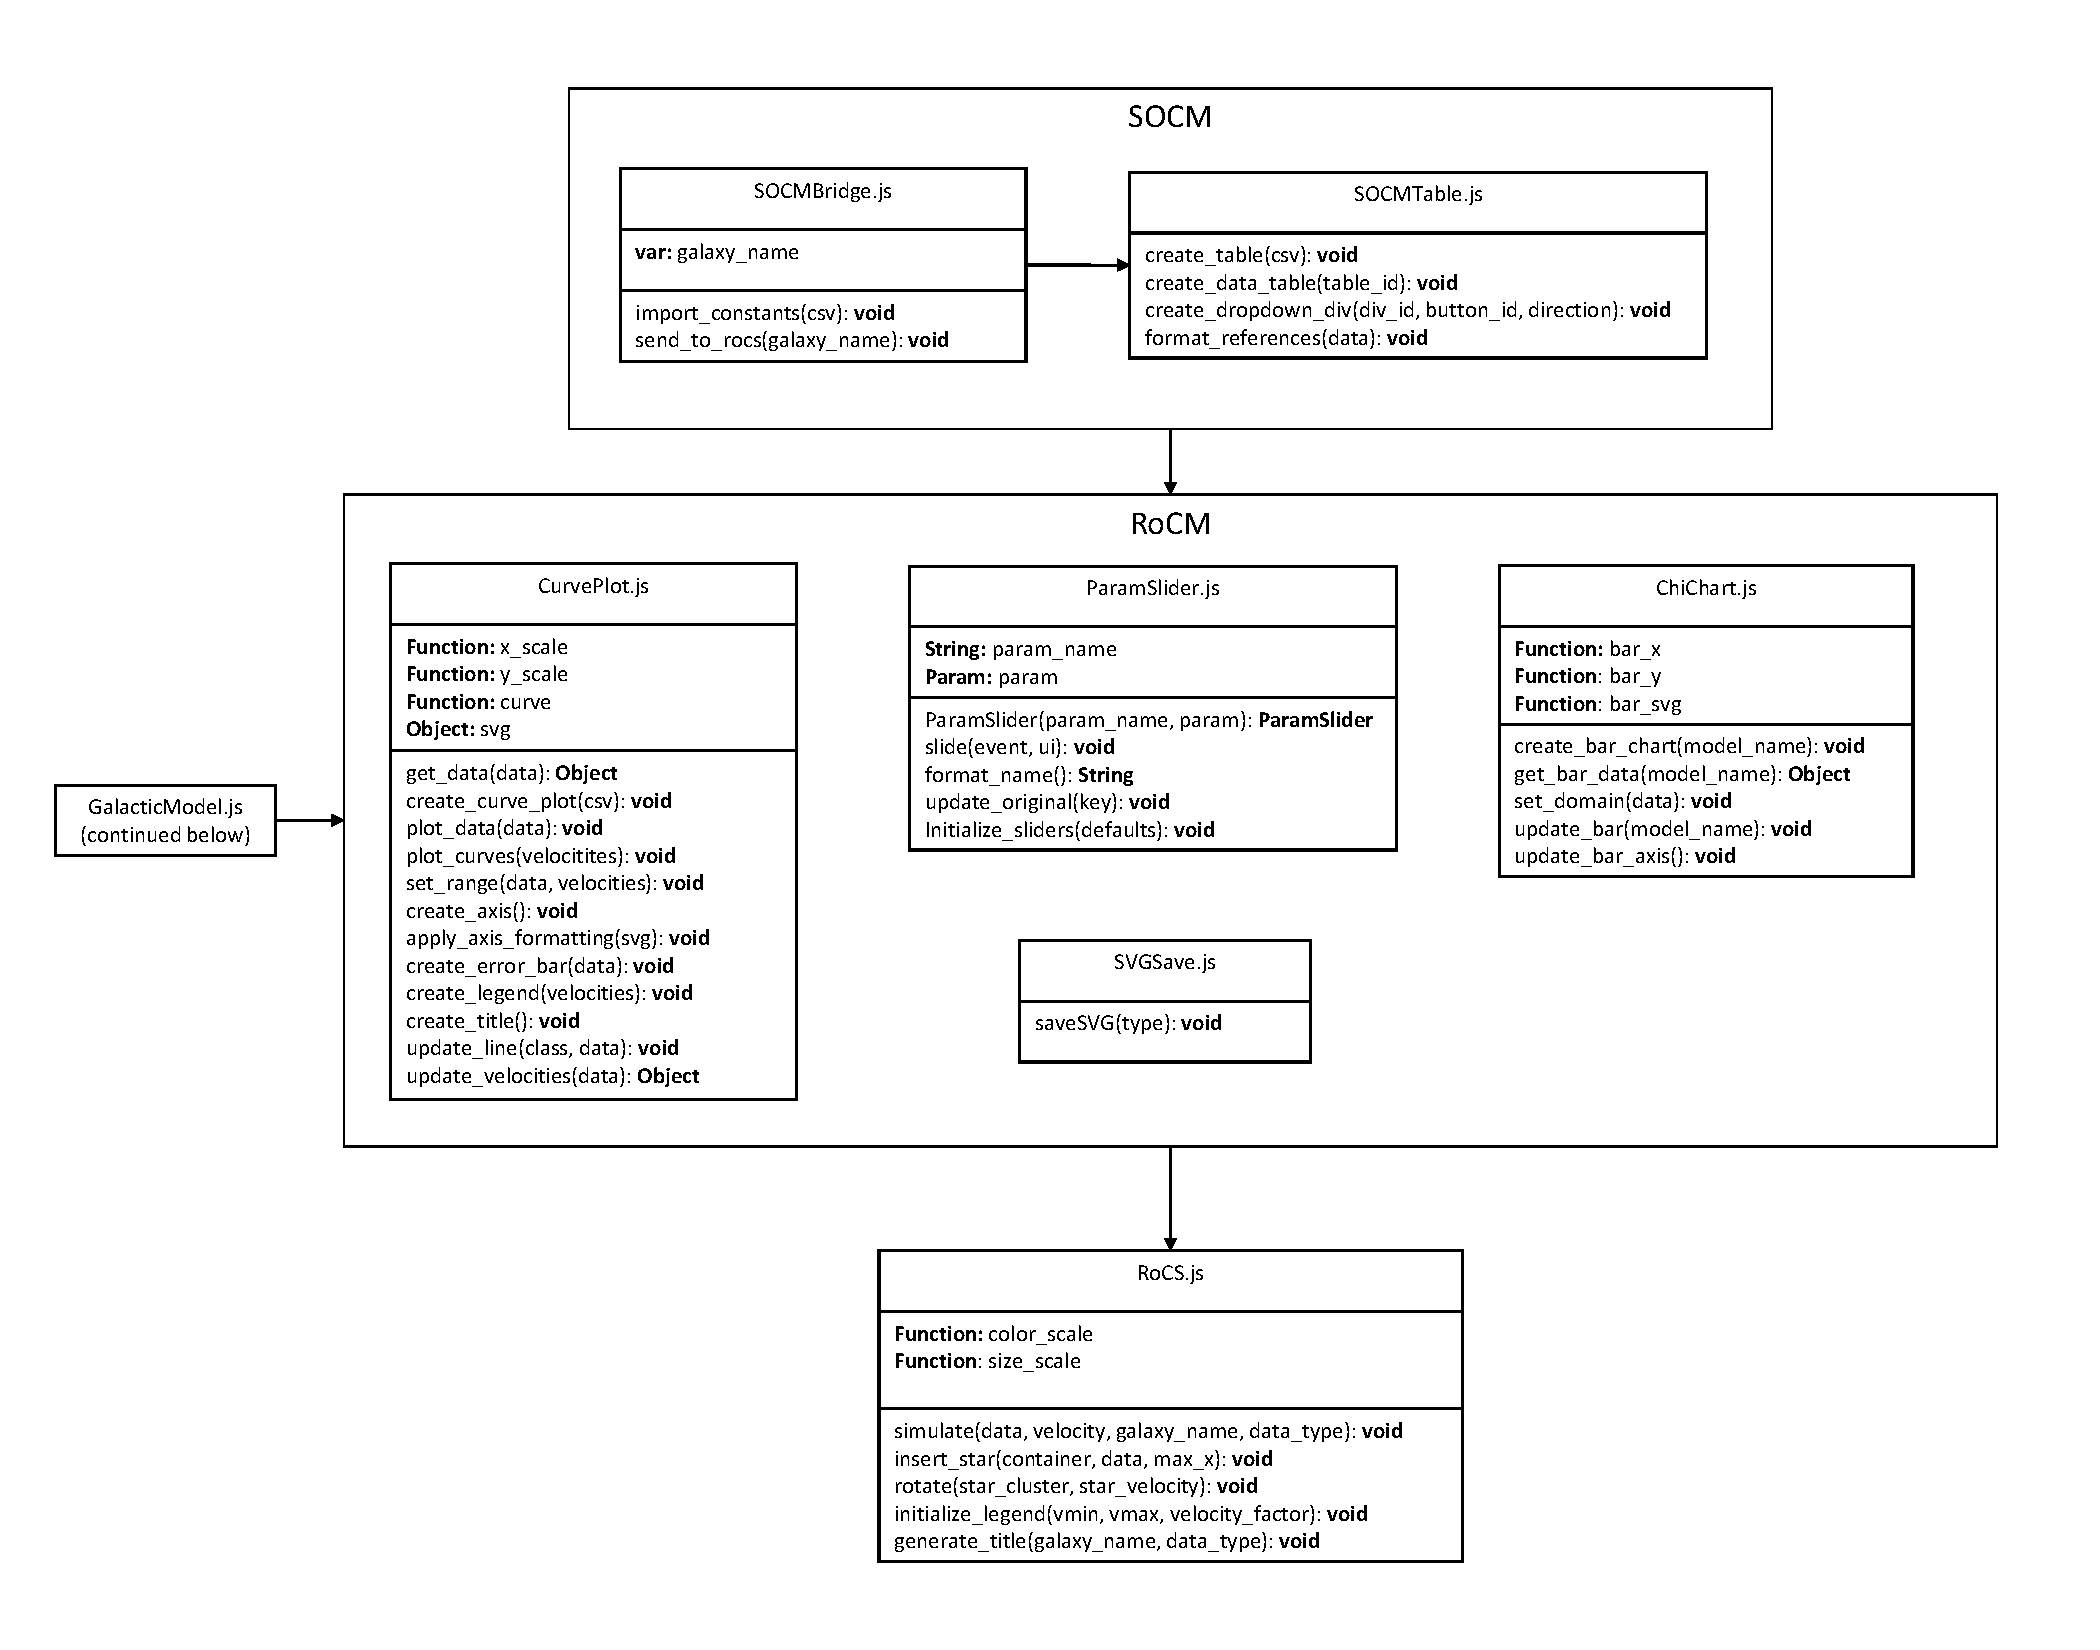
\includegraphics[width=\textwidth,height=\textheight,keepaspectratio]{decomposition_description_SOCMRoCMRoCS.pdf}

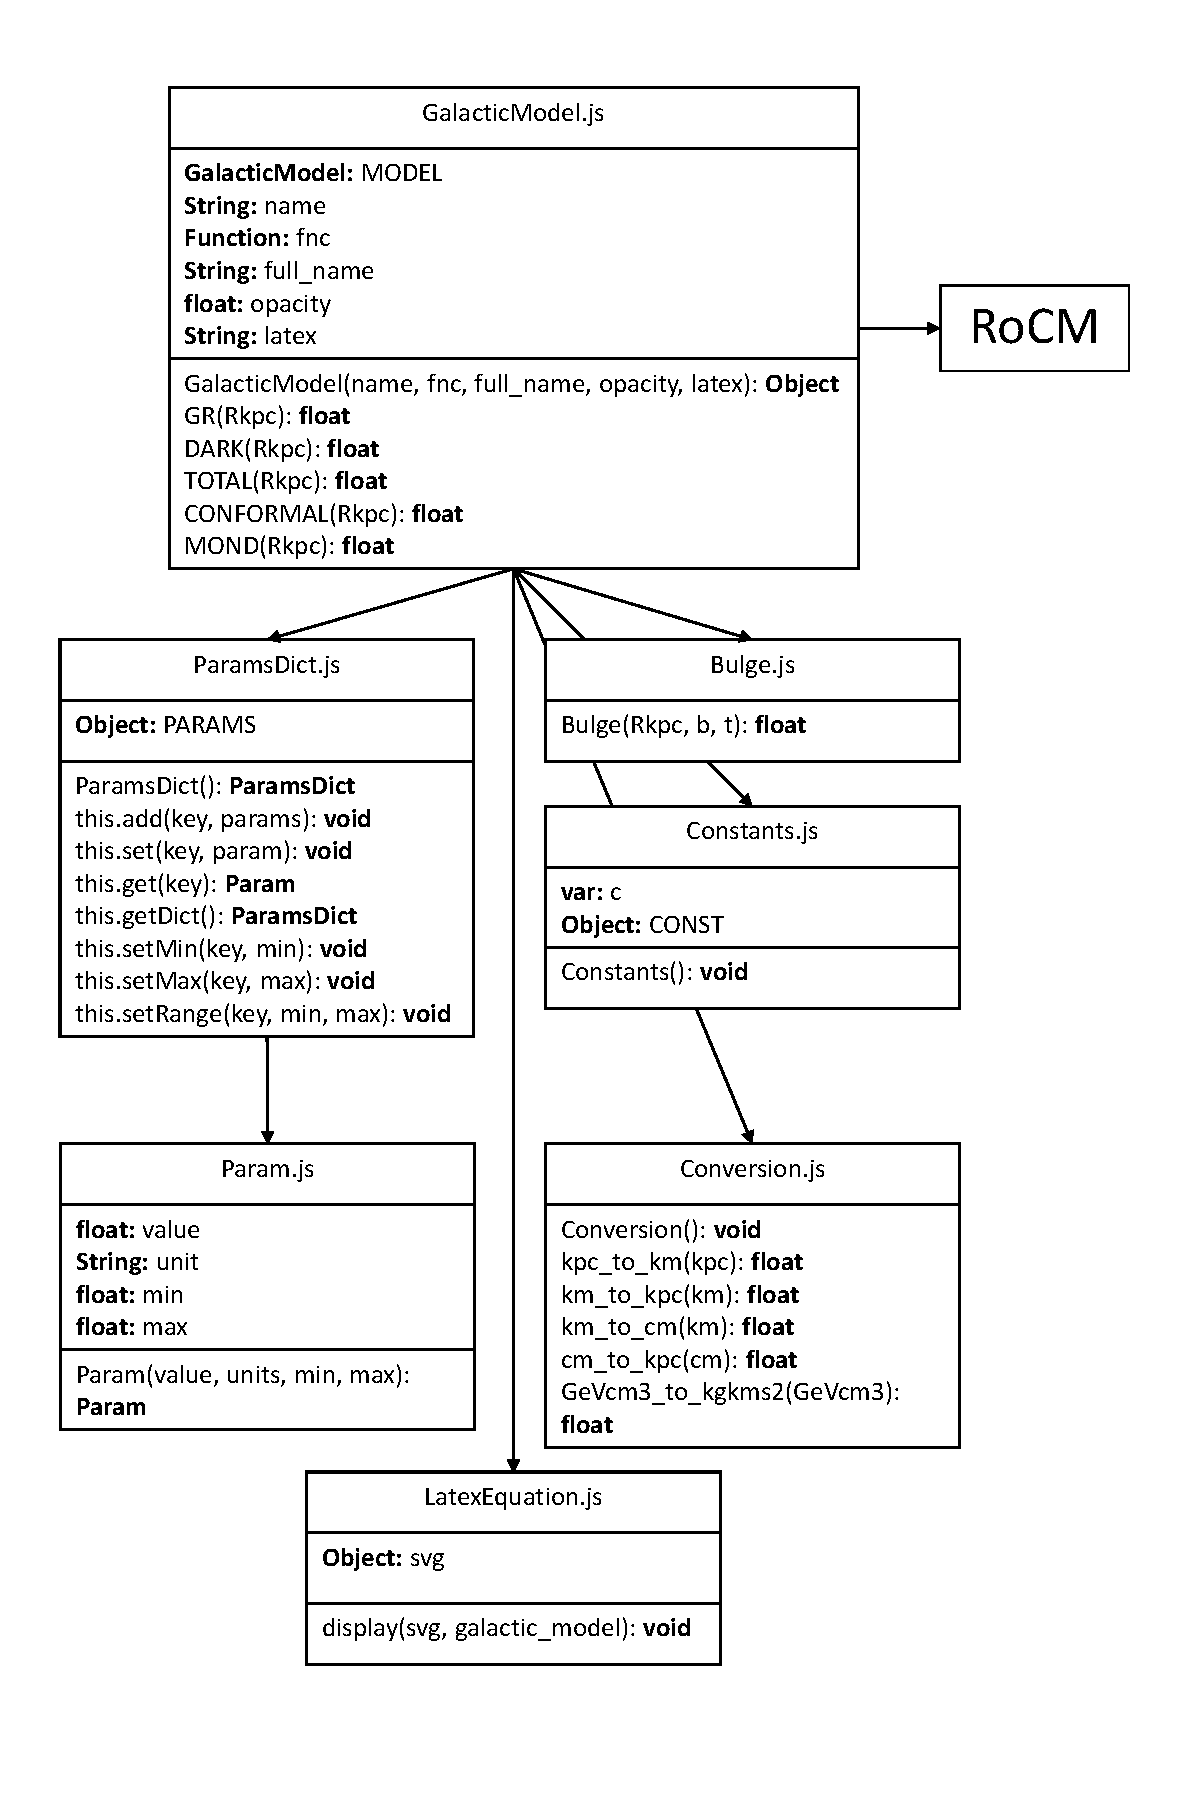
\includepdf[scale=0.75,pagecommand=\subsection{Class Diagram (Model Package)}]{decomposition_description_GalacticModel.pdf}

\subsection{Class Definition}
\subsubsection{CurvePlot}
CurvePlot will hold all of the graphing and plotting functions. It can import data from SOCM by calling \textit{get\_data(data)}. The imported data will need to be manipulated in order to generate a multi-line plot, this is done through \textit{update\_velocities(data)}. It then will dynamically create a graph, with ranges defined by \textit{set\_range(data, velocities)}. Each velocity curve will then be generated dynamically through the function call, \textit{plot\_curves(velocities)}. An interactive legend will also be generated with \textit{create\_legend(velocities)}. The \textit{x\_scale} and \textit{y\_scale} are static functions in the place of variables for scaling from pixels to (x,y) coordinates on the generated D3 graph.

\subsubsection{ChiChart}
The ChiChart histogram is an implementation of a $\chi^2$ (chi squared) distribution. This shows the validity of the model vs. the observed data. The ChiChart will get the data via \textit{get\_bar\_data(model\_name)}. After the data has been retrieved, the domain will be set (via \textit{set\_domain(data)}) and the bar will be updated with the current $\chi^2$ of the model vs. the observed data (via \textit{update\_bar(model\_name)}).

\subsubsection{ParamSlider}
Each ParamSlider will be created dynamically. All the slider needs to be created is an associative parameter name (one that is in PARAMS), and a Param object. The Param object has 4 fields: value, unit, min, and max. These dictate the value of the parameter, the units in which it's defined, and the min and max values of the ParamSlider. The \textit{slide(event, ui)} function will handle all the updating that needs to be done to the CurvePlot and ChiChart. The function \textit{update\_original(key)} can be used to reset the original value of the parameter.

\subsubsection{GalacticModel}
The GalacticModel object will reside in the global namespace. This global MODEL variable will have each implemented model as an indexable function (ex: MODEL["CONFORMAL"] will return the equation for Conformal Gravity. From here you can use that return object as the direct Confromal Gravity velocity function). Each defined model will have a name (short name for the model), the implemented equation (in the form of a v(R) function), a full name (full name of the model, for the legend), the opacity of the curve (optional), and the \LaTeX \- code of the equation (optional).

\end{document}